\documentclass{article}
\usepackage{amsmath}
\usepackage{tikz}
\usetikzlibrary{arrows.meta}

\begin{document}

\begin{center}
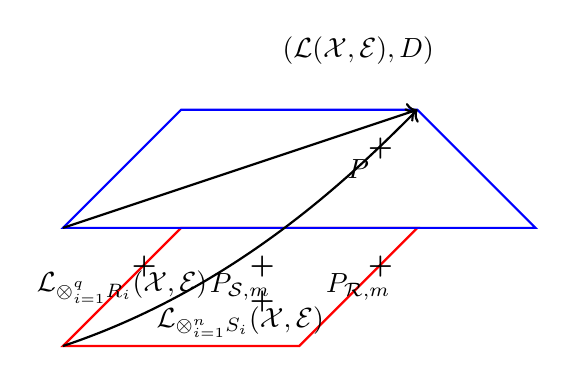
\begin{tikzpicture}[scale=1.5]
    % Define coordinates
    \coordinate (A) at (0,0);
    \coordinate (B) at (2,0);
    \coordinate (C) at (3,1);
    \coordinate (D) at (1,1);
    \coordinate (E) at (4,1);
    \coordinate (F) at (3,2);
    \coordinate (G) at (1,2);
    \coordinate (H) at (0,1);

    % Draw the main quadrilateral
    \draw[red, thick] (A) -- (B) -- (C) -- (D) -- cycle;
    \draw[blue, thick] (E) -- (F) -- (G) -- (H) -- cycle;

    % Draw the diagonal lines
    \draw[black, thick, ->] (A) .. controls (1.5, 0.5) and (2.5, 1.5) .. (F);
    \draw[black, thick, ->] (H) -- (F);

    % Label the points
    \node at (2.5, 1.5) {$P$};
    \node at (1.5, 0.5) {$P_{\mathcal{S},m}$};
    \node at (2.5, 0.5) {$P_{\mathcal{R},m}$};
    \node at (0.5, 0.5) {$\mathcal{L}_{\otimes_{i=1}^{q} R_i}(\mathcal{X},\mathcal{E})$};
    \node at (1.5, 0.2) {$\mathcal{L}_{\otimes_{i=1}^{n} S_i}(\mathcal{X},\mathcal{E})$};
    \node at (2.5, 2.5) {$(\mathcal{L}(\mathcal{X},\mathcal{E}), D)$};

    % Add plus signs
    \node at (2.5, 1.5) [above right] {\textbf{+}};
    \node at (1.5, 0.5) [above right] {\textbf{+}};
    \node at (2.5, 0.5) [above right] {\textbf{+}};
    \node at (0.5, 0.5) [above right] {\textbf{+}};
    \node at (1.5, 0.2) [above right] {\textbf{+}};
\end{tikzpicture}
\end{center}

Hierarchical decomposition of divergence in terms of orthogonal projections with respect to a partition $\mathcal{R}$ and its refinement $\mathcal{S}$.

\end{document}